%%%%%%%%%%%%%%%%%%%%%%%%%%%%%%%%%%%%%%%%%
% Programming/Coding Assignment
% LaTeX Template
%
% This template has been downloaded from:
% http://www.latextemplates.com
%
% Original author:
% Ted Pavlic (http://www.tedpavlic.com)
%
% Note:
% The \lipsum[#] commands throughout this template generate dummy text
% to fill the template out. These commands should all be removed when 
% writing assignment content.
%
% This template uses a Perl script as an example snippet of code, most other
% languages are also usable. Configure them in the "CODE INCLUSION 
% CONFIGURATION" section.
%
%%%%%%%%%%%%%%%%%%%%%%%%%%%%%%%%%%%%%%%%%

%----------------------------------------------------------------------------------------
%	PACKAGES AND OTHER DOCUMENT CONFIGURATIONS
%----------------------------------------------------------------------------------------

\documentclass{article}

\usepackage{fancyhdr} % Required for custom headers
\usepackage{lastpage} % Required to determine the last page for the footer
\usepackage{extramarks} % Required for headers and footers
\usepackage[usenames,dvipsnames]{color} % Required for custom colors
\usepackage{graphicx} % Required to insert images
\usepackage{listings} % Required for insertion of code
\usepackage{courier} % Required for the courier font
\usepackage{lipsum} % Used for inserting dummy 'Lorem ipsum' text into the template
\usepackage{url}
\newcommand{\quotes}[1]{``#1''}
% Margins
\topmargin=-0.45in
\evensidemargin=0in
\oddsidemargin=0in
\textwidth=6.5in
\textheight=9.0in
\headsep=0.25in

\linespread{1.1} % Line spacing

% Set up the header and footer
\pagestyle{fancy}
\lhead{\hmwkAuthorName} % Top left header
\chead{\hmwkClass\ (\hmwkClassInstructor\ \hmwkClassTime) \hmwkTitle} % Top center head
\rhead{\firstxmark} % Top right header
\lfoot{\lastxmark} % Bottom left footer
\cfoot{} % Bottom center footer
\rfoot{Page\ \thepage\ of\ \protect\pageref{LastPage}} % Bottom right footer
\renewcommand\headrulewidth{0.4pt} % Size of the header rule
\renewcommand\footrulewidth{0.4pt} % Size of the footer rule

\setlength\parindent{0pt} % Removes all indentation from paragraphs

%----------------------------------------------------------------------------------------
%	CODE INCLUSION CONFIGURATION
%----------------------------------------------------------------------------------------

\definecolor{MyDarkGreen}{rgb}{0.0,0.4,0.0} % This is the color used for comments
\lstloadlanguages{R} % Load Perl syntax for listings, for a list of other languages supported see: ftp://ftp.tex.ac.uk/tex-archive/macros/latex/contrib/listings/listings.pdf
\lstset{language=R, % Use Perl in this example
        frame=single, % Single frame around code
        basicstyle=\small\ttfamily, % Use small true type font
        keywordstyle=[1]\color{Blue}\bf, % Perl functions bold and blue
        keywordstyle=[2]\color{Purple}, % Perl function arguments purple
        keywordstyle=[3]\color{Blue}\underbar, % Custom functions underlined and blue
        identifierstyle=, % Nothing special about identifiers                                         
        commentstyle=\usefont{T1}{pcr}{m}{sl}\color{MyDarkGreen}\small, % Comments small dark green courier font
        stringstyle=\color{Purple}, % Strings are purple
        showstringspaces=false, % Don't put marks in string spaces
        tabsize=5, % 5 spaces per tab
        %
        % Put standard Perl functions not included in the default language here
        morekeywords={},
        %
        % Put Perl function parameters here
        morekeywords=[2]{on, off, interp},
        %
        % Put user defined functions here
        morekeywords=[3]{test},
       	%
        morecomment=[l][\color{Blue}]{...}, % Line continuation (...) like blue comment
        numbers=left, % Line numbers on left
        firstnumber=1, % Line numbers start with line 1
        numberstyle=\tiny\color{Blue}, % Line numbers are blue and small
        stepnumber=5 % Line numbers go in steps of 5
}

% Creates a new command to include a perl script, the first parameter is the filename of the script (without .pl), the second parameter is the caption
\newcommand{\rscript}[2]{
\begin{itemize}
\item[]\lstinputlisting[caption=#2,label=#1]{#1.R}
\end{itemize}
}

%----------------------------------------------------------------------------------------
%	DOCUMENT STRUCTURE COMMANDS
%	Skip this unless you know what you're doing
%----------------------------------------------------------------------------------------

% Header and footer for when a page split occurs within a problem environment
\newcommand{\enterProblemHeader}[1]{
\nobreak\extramarks{#1}{#1 continued on next page\ldots}\nobreak
\nobreak\extramarks{#1 (continued)}{#1 continued on next page\ldots}\nobreak
}

% Header and footer for when a page split occurs between problem environments
\newcommand{\exitProblemHeader}[1]{
\nobreak\extramarks{#1 (continued)}{#1 continued on next page\ldots}\nobreak
\nobreak\extramarks{#1}{}\nobreak
}

\setcounter{secnumdepth}{0} % Removes default section numbers
\newcounter{homeworkProblemCounter} % Creates a counter to keep track of the number of problems

\newcommand{\homeworkProblemName}{}
\newenvironment{homeworkProblem}[1][Problem \arabic{homeworkProblemCounter}]{ % Makes a new environment called homeworkProblem which takes 1 argument (custom name) but the default is "Problem #"
\stepcounter{homeworkProblemCounter} % Increase counter for number of problems
\renewcommand{\homeworkProblemName}{#1} % Assign \homeworkProblemName the name of the problem
\section{\homeworkProblemName} % Make a section in the document with the custom problem count
\enterProblemHeader{\homeworkProblemName} % Header and footer within the environment
}{
\exitProblemHeader{\homeworkProblemName} % Header and footer after the environment
}

\newcommand{\problemAnswer}[1]{ % Defines the problem answer command with the content as the only argument
\noindent\framebox[\columnwidth][c]{\begin{minipage}{0.98\columnwidth}#1\end{minipage}} % Makes the box around the problem answer and puts the content inside
}

\newcommand{\homeworkSectionName}{}
\newenvironment{homeworkSection}[1]{ % New environment for sections within homework problems, takes 1 argument - the name of the section
\renewcommand{\homeworkSectionName}{#1} % Assign \homeworkSectionName to the name of the section from the environment argument
\subsection{\homeworkSectionName} % Make a subsection with the custom name of the subsection
\enterProblemHeader{\homeworkProblemName\ [\homeworkSectionName]} % Header and footer within the environment
}{
\enterProblemHeader{\homeworkProblemName} % Header and footer after the environment
}

%----------------------------------------------------------------------------------------
%	NAME AND CLASS SECTION
%----------------------------------------------------------------------------------------

\newcommand{\hmwkTitle}{Homework\ \#0} % Assignment title
\newcommand{\hmwkDueDate}{Saturday Jan 22,  2022 16:00 p.m.}% Due date
\newcommand{\hmwkClass}{Introduction to Data Analysis and Mining\\} % Course/class
\newcommand{\hmwkClassTime}{} % Class/lecture time
\newcommand{\hmwkClassInstructor}{Instructor: Dr. H. Kurban} % Teacher/lecturer
\newcommand{\hmwkAuthorName}{Student Name} % Your name

%----------------------------------------------------------------------------------------
%	TITLE PAGE
%----------------------------------------------------------------------------------------

\title{
\vspace{2in}
\textmd{\textbf{\hmwkClass\ \hmwkTitle}}\\
\normalsize\vspace{0.1in}\small{Due\ on\ \hmwkDueDate}\\
\vspace{0.1in}\large{\textit{\hmwkClassInstructor\ }}
\vspace{3in}
}

\author{\textbf{\hmwkAuthorName}}
\date{\today} % Insert date here if you want it to appear below your name

%----------------------------------------------------------------------------------------

\begin{document}

\maketitle

%----------------------------------------------------------------------------------------
%	TABLE OF CONTENTS
%----------------------------------------------------------------------------------------

%\setcounter{tocdepth}{1} % Uncomment this line if you don't want subsections listed in the ToC

\newpage
%\tableofcontents
\newpage



%----------------------------------------------------------------------------------------
%	PROBLEM 1
%----------------------------------------------------------------------------------------

% To have just one problem per page, simply put a \clearpage after each problem
\begin{homeworkProblem}


 Here is data from the \textit{Digest of Education Statistics, 2005,Table 63.} -- viewed in a plain text file called \url{teach.txt}.  You are allowed to use R packages/Python libraries and built-in functions for this question.

\begin{table}[h]
\centering
\begin{tabular}{l} 
Year, Ratio \\
1955, 26.9 \\
1960, 25.8 \\
1965, 24.7 \\
1970, 22.3 \\
1980, 18.7 \\
1985, 17.9 \\
1990, 17.2 \\
1995, 117.3 \\
2000, 16.0 \\
2005, 15.5 \\
\end{tabular}
\end{table}

\begin{enumerate}
\item[\textbf{ Q1.1}] Provide the R/Python code that reads  the data from teach.txt into an \textsf{R}/Python data.frame?


\subsection{R script }
\begin{lstlisting}[language=R]
# Sample R Script With Highlighting

\end{lstlisting}


 \subsection{Python script}
\begin{lstlisting}[language=Python]
# Sample Python Script With Highlighting
\end{lstlisting}

\item[\textbf{ Q1.2}] Suppose you're interested in looking at \textit{only} the Ratios.  Give \textsf{R}/Python code that produces this data. 


\subsection{R script }
\begin{lstlisting}[language=R]
# Sample R Script With Highlighting

\end{lstlisting}


 \subsection{Python script}
\begin{lstlisting}[language=Python]
# Sample Python Script With Highlighting
\end{lstlisting}


\pagebreak

\item[\textbf{ Q1.3}]  Give a select operation on the data.frame that gives the rows whose ratios are greater than 18, but less than 22.  What does this yield?


\subsection{R script }
\begin{lstlisting}[language=R]
# Sample R Script With Highlighting

\end{lstlisting}


 \subsection{Python script}
\begin{lstlisting}[language=Python]
# Sample Python Script With Highlighting
\end{lstlisting}



\item[\textbf{ Q1.4}] Here is the histogram plot of \texttt{teach\$Ratio}
\begin{center}
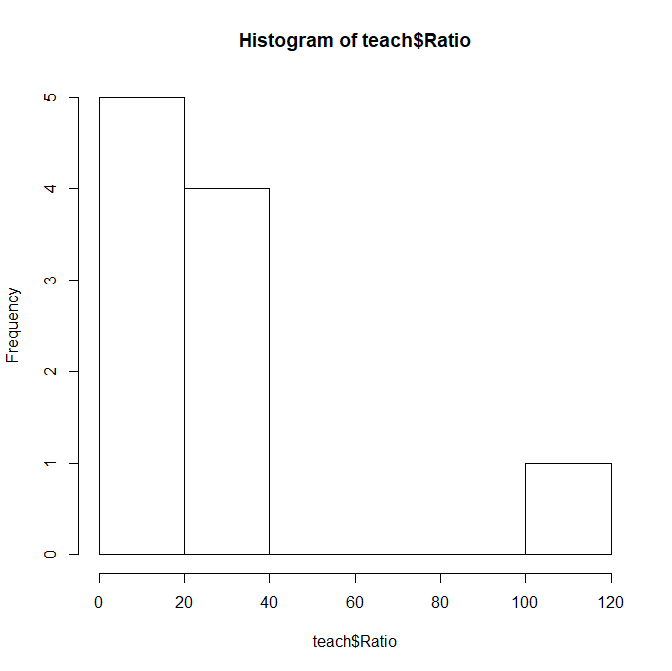
\includegraphics[width=10cm]{plote1.png} % Example image
\end{center}
Give \textsf{R}/Python code that produces this plot. 

\subsection{R script }
\begin{lstlisting}[language=R]
# Sample R Script With Highlighting

\end{lstlisting}


 \subsection{Python script}
\begin{lstlisting}[language=Python]
# Sample Python Script With Highlighting
\end{lstlisting}





\end{enumerate}

\end{homeworkProblem}

%----------------------------------------------------------------------------------------
%	PROBLEM 2
%----------------------------------------------------------------------------------------


\begin{homeworkProblem}
 Load mydata.txt into R/Python and answer the following questions. You are allowed to use R/Python packages and built-in functions for this question.
\begin{enumerate}
\item[Q2.1] How many entries are there in the data set? Answer here \ldots


\subsection{R script }
\begin{lstlisting}[language=R]
# Sample R Script With Highlighting

\end{lstlisting}


 \subsection{Python script}
\begin{lstlisting}[language=Python]
# Sample Python Script With Highlighting
\end{lstlisting}




\item[Q2.2] Calculate mean and median of variable V2. Answer here \ldots


\subsection{R script }
\begin{lstlisting}[language=R]
# Sample R Script With Highlighting

\end{lstlisting}


 \subsection{Python script}
\begin{lstlisting}[language=Python]
# Sample Python Script With Highlighting
\end{lstlisting}


\item[Q2.3] Find variance and standard deviation  of variable V1. Answer here \ldots
\subsection{R script }
\begin{lstlisting}[language=R]
# Sample R Script With Highlighting

\end{lstlisting}


 \subsection{Python script}
\begin{lstlisting}[language=Python]
# Sample Python Script With Highlighting
\end{lstlisting}

\item[Q2.4] Variable 5, $V5$, is the class variable and the bar plot below shows the distribution of data points among different classes. Give the R /Python code that produces the  figure below. (Color is not required to be the same)

\begin{center}
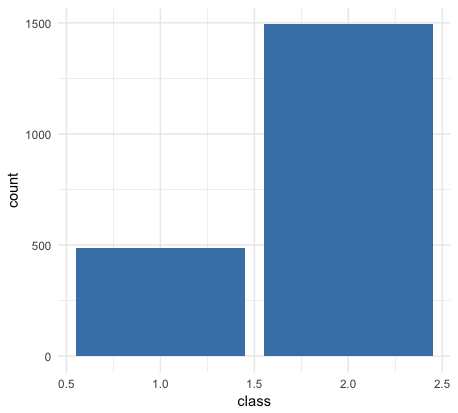
\includegraphics[width=10cm]{barplot1.png} % Example image
\end{center}


\subsection{R script }
\begin{lstlisting}[language=R]
# Sample R Script With Highlighting

\end{lstlisting}


 \subsection{Python script}
\begin{lstlisting}[language=Python]
# Sample Python Script With Highlighting
\end{lstlisting}


\end{enumerate}
\end{homeworkProblem}

%----------------------------------------------------------------------------------------
%	PROBLEM 3
%----------------------------------------------------------------------------------------
\begin{homeworkProblem}
Create an R/a Python function that calculates Euclidean distance between same dimensional  two vectors (data points). Call this function dist.euclidean.R.  Assume three pieces of data $x_1 = (1,2); x_2 = (3,4); x_3 = (6,4)$ ($x_1, x_2, x_3$ are two dimensional data points).  Using your R function, determine which two are the least dissimilar. Answer here \ldots.



\subsection{R script }
\begin{lstlisting}[language=R]
# Sample R Script With Highlighting

\end{lstlisting}


 \subsection{Python script}
\begin{lstlisting}[language=Python]
# Sample Python Script With Highlighting
\end{lstlisting}

\end{homeworkProblem}

\pagebreak
%----------------------------------------------------------------------------------------
%	PROBLEM 4
%----------------------------------------------------------------------------------------
\begin{homeworkProblem}

In this question, you are asked to implement two R/Python functions to calculate mean and variance.  Call this functions sample.mean.R and sample.variance.R. You're given a sample of data: 15,2,44,21,40,20,19,18.  Calculate the sample mean and sample variance using your functions. Answer here$\ldots$
%%%%%%%%%%%%%%%%%%%%%%%%%%%%%%%%%%

\subsection{R script }
\begin{lstlisting}[language=R]
# Sample R Script With Highlighting

\end{lstlisting}


 \subsection{Python script}
\begin{lstlisting}[language=Python]
# Sample Python Script With Highlighting
\end{lstlisting}

\end{homeworkProblem}
%----------------------------------------------------------------------------------------


 



\end{document}